\documentclass[../SimBALink.tex]{subfiles}
\begin{document}
\section{Vehicle} This system models the forces acting on the vehicle.
\begin{figure}[H]
  \centering
  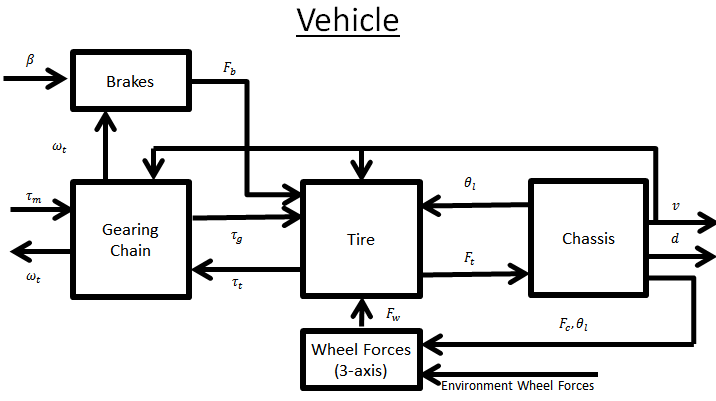
\includegraphics[scale=.75]{Vehicle_Diagram}
  \caption{Vehicle Diagram}
\end{figure}
\subfile{./Docs/Chain_Gear}
\subfile{./Docs/Brakes}
\subfile{./Docs/Tires}
\subfile{./Docs/Wheel_Forces}
\subfile{./Docs/Chassis}

\subsection{Validation}
A PI controller was added to the vehicle model as a whole to control for speed. The test shows the vehicle starting at 20 m/s and going to 40 m/s. The model works well.

\begin{figure}[H]
  \centering
  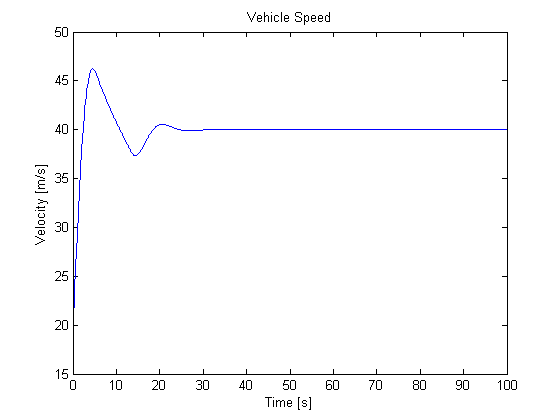
\includegraphics[scale= 1]{veh_val_speed}
  \caption{Vehicle Validation Speed}
\end{figure}

\begin{figure}[H]
  \centering
  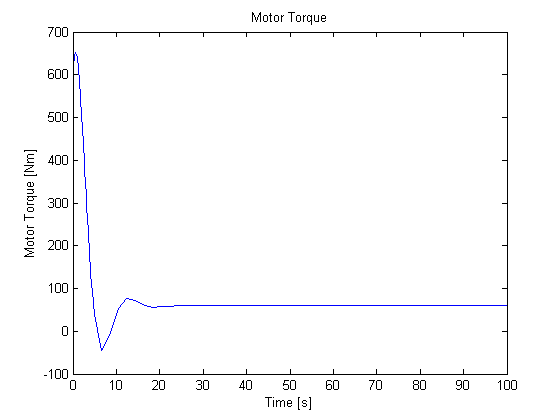
\includegraphics[scale=1]{veh_val_motor}
  \caption{Vehicle Validation Motor Torque}
\end{figure}

\begin{figure}[H]
  \centering
  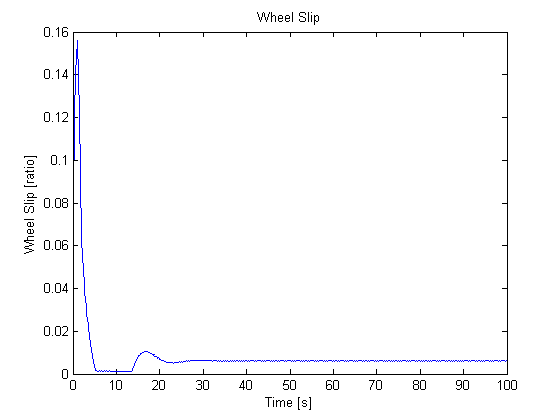
\includegraphics[scale=1]{veh_val_slip}
  \caption{Vehicle Validation Slip}
\end{figure}

The Model was also validated with coastdown data by making the command velocity 0.

\begin{figure}[H]
  \centering
  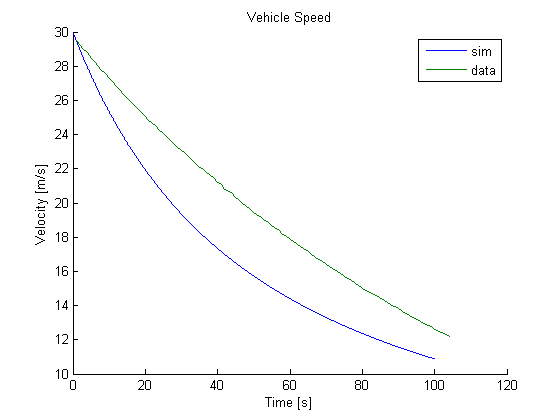
\includegraphics[scale=1]{veh_val_coastdown}
  \caption{Vehicle Validation Coastdown}
\end{figure}

\end{document}